\documentclass[xcolor=dvipsnames]{beamer}

    % short version in [], full version in {}.
    \title[pre]{Presentation in \LaTeX}
    \subtitle[pre by zcc]{Presented by Charlie Zhao}
    \author[zcc]{Charlie Zhao}
    \date[2018]{\today}
    \institute[SJTU]{Shanghai Jiao Tong University}

    % set the main color for the ppt.
    \usecolortheme[named=Maroon]{structure}
    % set ppt theme (e.g. Boadilla, Singapore, Warsaw).
    \usetheme{Boadilla}

    \usepackage{package}

    \begin{document}

        % every piece of slide is displayed in the form of frame.
        % t to place at the top.
        % b to place at the bottom.
        % c to place at the center.
        \begin{frame}[t]
            \titlepage
        \end{frame}

        \begin{frame}[t]
            \frametitle{Outline}
            \tableofcontents
        \end{frame}

        \section{slide1}
        \begin{frame}[t]

            \frametitle{Neural Networks}
            There are many kinds of neural networks.

            % insert bulletin points to the slide.
            \begin{itemize}
                \item CNN
                \item RNN
                \item LSTM
            \end{itemize}

        \end{frame}

        \section{slide2}
        \begin{frame}[t]

            \frametitle{Neural Networks 2}
            More...

            % insert list to the slide.
            \begin{enumerate}
                \item CNN
                \item RNN
                \item LSTM
            \end{enumerate}

        \end{frame}

        \section{slide3}
        \begin{frame}[t]

            \frametitle{The Universe}

            \begin{figure}[h!]
                \centering
                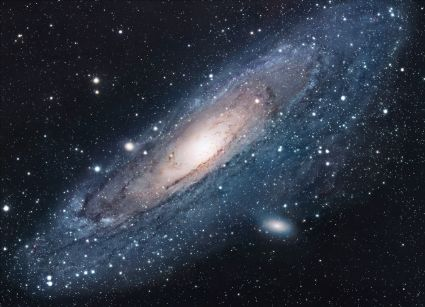
\includegraphics[scale=1.7]{universe.jpg}
                \caption{The Universe}
                \label{universe}
                % use \pause for present the rest of the slide at the next click.
                \pause
            \end{figure}

            \begin{enumerate}
                \item CNN
                \item RNN
                \item LSTM
            \end{enumerate}

        \end{frame}

        \section{slide4}
        \begin{frame}[t]

            \frametitle{A Table of $\pi$}

            % insert a table to the slide.
            % |c| indicates center of each blank.
            \centering
            \begin{tabular}{|c|c|c|c|} \hline
                1 & 2 & 3 & 4 \\ \hline
                3.1 & 3.14 & 3.141 & 3.1415 \\ \hline
            \end{tabular}

            \begin{enumerate}
                % use \centering in the structure to center the structure.
                % also use \begin{center} and \end{center}.
                \centering
                \item CNN
                \item RNN
                \item LSTM
            \end{enumerate}

        \end{frame}

    \end{document}